\section{\secperms}
\label{sec_perms}

% An ancient \textbf{cipher} (secret code) replaces each letter ($A-Z$) with another in a cyclic fashion. For example, we could replace each letter by three letters later: $$A \to D, B \to E, C \to F, \ldots, W \to Z, X \to A, Y \to B,\text{ and }Z \to C$$   
% Under this cipher $MATHEMATICS \to PDWKHPDWLV$.  If you have ever solved Cryptoquips or other cryptogram puzzles, you know that single letter replacement code can be solved, and often rather quickly.  Cyclic codes are even easier because once you figure out one letter the rest follow. Modern encryption algorithms use much fancier mathematics to create really difficult to solve ciphers. One key ingredient to modern encryption is rearranging the order of letters (or strings of symbols).  Mathematically, such a reordering is called a \textbf{permutation}. \bigskip

We start this section by looking at permutations, which are bijections between a set and itself, and discuss the composition of permutations.  Next, building on our examples with permutations, we define function composition and function inverses, in general. Lastly, we explore how to prove that a function is one-to-one and, more generally, a proof format for uniqueness proofs as well as existence and uniqueness proofs.

%%%%%%%%%%%%%%%%%%%%%%%%
\newcommand{\subperms}{Permutations}
\subsection{\subperms}
\label{sub_permutations}

Permutations are used in many applications. For example, they are used to describe the shuffling of a deck of cards, analyze sorting algorithms, and model gene sequencing.  They are used in encryption and error-correction algorithms and for games such as anagrams, the sliding 15 puzzle, and Rubik's Cube{\texttrademark}.  We start with the definition.

\begin{defn}[Permutation]
\label{defn_permutation}
~    
    \begin{apart}
        \item A \vocab{permutation} is a function $f:X \to X$ for some set $X$ such that $f$ is onto and one-to-one. In other words, a permutation is a bijection from a set to itself. Equivalently, a permutation is a function whose rule is a pairing of a set with itself. For example, the function $h: \mathbb{R} \to \mathbb{R}$ defined by $h(x) = 3x$ is a permutation, as we saw in \Cref{exam_bijections}.
        \item We are often interested in a permutation of the set $\{1,2,\ldots,n\}$ for some positive integer $n$.  We can describe such permutations by listing the values, drawing the standard dot diagram, or using \vocab{2-line notation}
            $$\alpha = 
            \left(\begin{array} {ccc cc}
            1 & 2 & 3 & \ldots & n \\
            \alpha(1) & \alpha(2) & \alpha(3) & \ldots & \alpha(n) 
            \end{array} \right)$$
        For example, if $\sigma: \{1,2,3,4\} \to \{1,2,3,4\}$ is the permutation defined by $\sigma(1)=2$, $\sigma(2)=3$, $\sigma(3)=4$, and $\sigma(4)=1$, then we write 
            $$\sigma = 
            \left(\begin{array} {ccc c}
            1 & 2 & 3 & 4 \\
            2 & 3 & 4 & 1
            \end{array} \right).$$
        In the 2-line notation, the first line is always $1 2 3 \ldots n$ and the second line contains each of $1, 2, 3, \ldots, n$ exactly once.
    \end{apart}  
\end{defn}

Permutations are often named with lowercase Greek letters.

\begin{rem}[Greek letters]
\label{rem_Greek_letters}
    \Cref{table_lowercase_greek} lists a few lowercase Greek letters commonly used for permutations.
        \begin{table}[hbtp]
            \centering
            \begin{tabular}{cccccc}
                $\alpha=$ alpha & 
                $\beta=$ beta &
                $\gamma=$ gamma & 
                $\delta=$ delta & 
                $\epsilon=$ epsilon &
                $\mu=$ mu  \\
                $\nu=$ nu &
                $\rho=$ rho &
                $\sigma=$ sigma &
                $\tau=$ tau &
                $\psi=$ psi &
                $\chi=$ chi 
            \end{tabular}
            \caption{A few lowercase Greek letters commonly used for permutations.}
            \label{table_lowercase_greek}
        \end{table}
\end{rem}

Let's look more closely at permutations on $\{1,2,3,4\}$.

\begin{exam}[Permutations on $\{1,2,3,4\}$]
\label{exam_perm_fns1234}   
~
    \begin{apart}
        \item Draw the dot diagram for the permutation 
        $\sigma = \left(\begin{array} {ccc c}
            1 & 2 & 3 & 4 \\
            2 & 3 & 4 & 1
        \end{array} \right).$
            \begin{soln}
                    \Cref{fig_perm_sigma} shows two versions of the dot diagram -- the standard version on the left and an unlabeled version on the right.
            \end{soln}
            \begin{figure}[hbtp]
                \centering
                \input{Tikz/perm_1234_sigma}
                \caption{The dot diagram and unlabeled dot diagram for $\sigma = \left(\begin{array} {ccc c}
            1 & 2 & 3 & 4 \\
            2 & 3 & 4 & 1
        \end{array} \right)$.}
                \label{fig_perm_sigma}
            \end{figure}
        \item Is the identity function a permutation on $\{1,2,3,4\}$?
            \begin{soln}
                The identity permutation $i: \{1,2,3,4\} \to \{1,2,3,4\}$ is defined by $i(n)=n$.  \Cref{fig_perm_id} shows the dot diagram of $i$.  Since the function $i$ is both onto and one-to-one with domain and codomain of $\{1,2,3,4\}$, the identity function $i$ is a permutation.  We can write 
                    $$i = \left(\begin{array} {ccc c}
                    1 & 2 & 3 & 4 \\
                    1 & 2 & 3 & 4
                    \end{array} \right).$$
            \end{soln}
            \begin{figure}[hbtp]
                \centering
                %Used in \Cref{sec_onetoone_onto_fns}.

\begin{tikzpicture}
[scale =.35]
\GraphInit[vstyle=Welsh]
\SetUpEdge[style={->,>=triangle 45}]
\SetGraphUnit{1.6}
%\SetVertexNoLabel
\Vertex[LabelOut,Lpos=180,x=0,y=6] {$1$}
\Vertex[LabelOut,Lpos= 180,x=0,y=4]{$2$}
\Vertex[LabelOut,Lpos=180,x=0,y=2]{$3$}
\Vertex[LabelOut,Lpos=180,x=0,y=0]{$4$}
\Vertex[LabelOut,Lpos=0,x=4,y=6]{$ 1$}
\Vertex[LabelOut,Lpos= 0,x=4,y=4]{$ 2$}
\Vertex[LabelOut,Lpos=0,x=4,y=2]{$ 3$}
\Vertex[LabelOut,Lpos=0,x=4,y=0]{$ 4$}
\Edges($1$,$ 1$)
\Edges($2$,$ 2$)
\Edges($3$,$ 3$)
\Edges($4$,$ 4$)
\end{tikzpicture}
\hspace{1in}
\begin{tikzpicture}
[scale =.35]
\GraphInit[vstyle=Welsh]
%\SetUpEdge[style={->,>=triangle 45}]
\SetGraphUnit{1.6}
\SetVertexNoLabel
\Vertex[LabelOut,Lpos=180,x=0,y=6] {$1$}
\Vertex[LabelOut,Lpos= 180,x=0,y=4]{$2$}
\Vertex[LabelOut,Lpos=180,x=0,y=2]{$3$}
\Vertex[LabelOut,Lpos=180,x=0,y=0]{$4$}
\Vertex[LabelOut,Lpos=0,x=4,y=6]{$ 1$}
\Vertex[LabelOut,Lpos= 0,x=4,y=4]{$ 2$}
\Vertex[LabelOut,Lpos=0,x=4,y=2]{$ 3$}
\Vertex[LabelOut,Lpos=0,x=4,y=0]{$ 4$}
\Edges($1$,$ 1$)
\Edges($2$,$ 2$)
\Edges($3$,$ 3$)
\Edges($4$,$ 4$)
\end{tikzpicture}

                \caption{The dot diagram and unlabeled dot diagram for $i = \left(\begin{array} {ccc c}
                1 & 2 & 3 & 4 \\
                1 & 2 & 3 & 4
                \end{array} \right)$.}
                \label{fig_perm_id}
            \end{figure}
        \item How many permutations on $\{1,2,3,4\}$ are there? Explain how you count.
            \begin{soln}
                There are four choices for where the permutation maps one.  Since permutations are one-to-one, there are three choices left for where the permutation maps two. Similarly, there are only two choices left for where the permutation maps three and then one choice for where the permutation maps four.  Therefore there are $4!$ permutations on the set $\{1,2,3,4\}$.
            \end{soln}
    \end{apart}
\end{exam}

In \Cref{exam_perm_fns1234}, we drew an unlabeled version of the dot diagrams where we omitted the vertex labels (always 1, 2, \ldots $n$ from top to bottom) and the arrows (always left-to-right).  The unlabeled version can save writing and so we use it in our examples, but feel free to stick with the standard dot diagram if you prefer.

There is a natural way to combine permutations.

\begin{defn}[Permutation composition]
\label{defn_perm_composition}
~
    \begin{apart}
        \item For any permutations $\alpha$ and $\beta$ on $\{1,2,3, \ldots,n\}$, their \textbf{composite} $\gamma$ is defined by $\gamma(x) = \alpha(\beta(x))$.  We often write $\alpha \circ \beta$ instead of $\gamma$; that is, $(\alpha \circ \beta)(x) = \alpha(\beta(x))$. Notice in the composite $\alpha \circ \beta$ that $\beta$ is applied first and $\alpha$ is applied second, which feels backward but is correct.  For example, let
            $$\sigma = \left ( \begin{array} {cccc} 1 & 2 & 3 & 4 \\ 2 & 3 & 4 & 1  \end{array} \right ) \text{ and } \tau= \left ( \begin{array} {cccc} 1 & 2 & 3 & 4\\ 2 & 1 & 4 & 3  \end{array} \right ).$$
       Then 
            $$\sigma \circ \tau = \left ( \begin{array} {cccc} 1 & 2 & 3 & 4 \\ 3 & 2 & 1 & 4 \end{array} \right ),$$ 
        as we see in \Cref{exam_composing_perms}.

        \item For a permutation $\alpha$, the \vocab{($n$th) iterate} of $\alpha$ is the composite 
            $$\alpha^n=\underbrace{\alpha \circ \alpha \circ \alpha \cdots \circ \alpha}_{n \text{ times}}.$$
        For example, for that permutation $\sigma$, it turns out that 
            $$\sigma^2=\sigma \circ \sigma = \left ( \begin{array} {cccc} 1 & 2 & 3 & 4 \\ 3 & 4 & 1 & 2  \end{array} \right ),$$ 
        as we see in \Cref{exam_composing_perms}.
    \end{apart}
\end{defn}

Let's check the examples from \Cref{defn_perm_composition}.

\begin{exam}[Composing permutations]
\label{exam_composing_perms}
    Consider the permutations   
        $$\sigma = \left ( \begin{array} {cccc} 1 & 2 & 3 & 4 \\ 2 & 3 & 4 & 1 \\ \end{array} \right ) \text{ and }
        \tau= \left ( \begin{array} {cccc} 1 & 2 & 3 & 4\\ 2 & 1 & 4 & 3 \end{array} \right ).$$
            \begin{apart}
                \item \label{part_sigma_of_tau} Calculate $\sigma \circ \tau$.
                    \begin{soln}
                        We have
                            \begin{align*}
                                (\sigma \circ \tau)(1) &= \sigma(\tau(1))=\sigma(2)=3  \\
                                (\sigma \circ \tau)(2) &= \sigma(\tau(2))=\sigma(1)=2 \\
                                (\sigma \circ \tau)(3) &= \sigma(\tau(3))=\sigma(4)=1 \\
                                (\sigma \circ \tau)(4) &= \sigma(\tau(4))=\sigma(3)=4 \\
                            \end{align*}
                        Thus $$\sigma \circ \tau = \left ( \begin{array} {cccc} 1 & 2 & 3 & 4 \\ 3 & 2 & 1 & 4 \end{array} \right ).$$
                        There is a quicker way to compute this composite using the unlabeled dot diagrams shown in \Cref{fig_sigma_of_tau}.  To read this diagram, start with the uppermost dot on the left which represents 1.  Moving right, follow the path to end on the third dot on the right which represents 3.  Thus the composite maps 1 to 3.  Repeat with each dot on the left following the path.
                    \begin{figure}[hbtp]
                        \centering
                        %Used in \Cref{sec_onetoone_onto_fns}.

\begin{tikzpicture}
[scale =.35]
\GraphInit[vstyle=Welsh]
%\SetUpEdge[style={->,>=triangle 45}]
\SetGraphUnit{1.6}
\SetVertexNoLabel
%%
\node at (2,8) {$\tau$};
\node at (6,8) {$\sigma$};
%%
\Vertex[LabelOut,Lpos=180,x=0,y=6]{$1$}
\Vertex[LabelOut,Lpos= 180,x=0,y=4]{$2$}
\Vertex[LabelOut,Lpos=180,x=0,y=2]{$3$}
\Vertex[LabelOut,Lpos=180,x=0,y=0]{$4$}
%%
\Vertex[LabelOut,Lpos=0,x=4,y=6]{$ 1$}
\Vertex[LabelOut,Lpos= 0,x=4,y=4]{$ 2$}
\Vertex[LabelOut,Lpos=0,x=4,y=2]{$ 3$}
\Vertex[LabelOut,Lpos=0,x=4,y=0]{$ 4$}
%%
\Vertex[LabelOut,Lpos=0,x=8,y=6]{$ 1 $}
\Vertex[LabelOut,Lpos= 0,x=8,y=4]{$ 2 $}
\Vertex[LabelOut,Lpos=0,x=8,y=2]{$ 3 $}
\Vertex[LabelOut,Lpos=0,x=8,y=0]{$ 4 $}
%%
\Edges($1$, $ 2$)
\Edges($2$, $ 1$)
\Edges($3$, $ 4$)
\Edges($4$, $ 3$)
%%
\Edges($ 1$, $ 2 $)
\Edges($ 2$, $ 3 $)
\Edges($ 3$, $ 4 $)
\Edges($ 4$, $ 1 $)
\end{tikzpicture}
%\hspace{.25in} %%%%%
\begin{tikzpicture}
[scale =.35]
\GraphInit[vstyle=Welsh]
%\SetUpEdge[style={->,>=triangle 45}]
\SetGraphUnit{1.6}
\SetVertexNoLabel
%%
\node at (2,8) {$\sigma \circ \tau$};
\node at (-2,3) {$=$};
%%
\Vertex[LabelOut,Lpos=180,x=0,y=6]{$1$}
\Vertex[LabelOut,Lpos= 180,x=0,y=4]{$2$}
\Vertex[LabelOut,Lpos=180,x=0,y=2]{$3$}
\Vertex[LabelOut,Lpos=180,x=0,y=0]{$4$}
%%
\Vertex[LabelOut,Lpos=0,x=4,y=6]{$ 1$}
\Vertex[LabelOut,Lpos= 0,x=4,y=4]{$ 2$}
\Vertex[LabelOut,Lpos=0,x=4,y=2]{$ 3$}
\Vertex[LabelOut,Lpos=0,x=4,y=0]{$ 4$}
%%
\Edges($1$, $ 3$)
\Edges($2$, $ 2$)
\Edges($3$, $ 1$)
\Edges($4$, $ 4$)
\end{tikzpicture}


                        \caption{The unlabeled dot diagram used to compute $\sigma \circ \tau$ from \Cref{exam_composing_perms} (\ref{part_sigma_of_tau}).}
                        \label{fig_sigma_of_tau}
                    \end{figure}
                    \end{soln}
                \item \label{part_tau_of_sigma} Calculate $\tau \circ \sigma$.
                    \begin{soln}
                        Following the paths in \Cref{fig_tau_of_sigma} we get 
                        $$\tau \circ \sigma = \left ( \begin{array} {cccc} 1 & 2 & 3 & 4 \\ 1 & 4 & 3 & 2 \end{array} \right ).$$
                Notice that the order mattered, in that $\sigma \circ \tau \ne \tau \circ \sigma$.  That is, composition of permutations is not commutative.
                    \begin{figure}[hbtp]
                        \centering
                        \input{Tikz/perm_comp_tau_of_sigma}
                        \caption{The unlabeled dot diagram used to compute $\tau \circ \sigma$ from \Cref{exam_composing_perms} (\ref{part_tau_of_sigma}).}
                        \label{fig_tau_of_sigma}
                    \end{figure}
                    \end{soln}
                \item \label{part_sigma_sq} Calculate $\sigma^2=\sigma \circ \sigma$.
                    \begin{soln}
                        Following the paths in \Cref{fig_sigma_sq} we get 
                        $$\sigma^2=\sigma \circ \sigma = \left ( \begin{array} {cccc} 1 & 2 & 3 & 4 \\ 3 & 4 & 1 & 2 \end{array} \right ).$$
                    \begin{figure}[hbtp]
                        \centering
                        \input{Tikz/perm_comp_sigma_sq}
                        \caption{The unlabeled dot diagram used to compute $\sigma \circ \sigma$ from \Cref{exam_composing_perms} (\ref{part_sigma_sq}).}
                        \label{fig_sigma_sq}
                    \end{figure}
                    \end{soln}
                \item \label{part_tau_sq} Calculate $\tau^2=\tau \circ \tau$.
                    \begin{soln}
                        Following the paths in \Cref{fig_tau_sq} we get 
                        $$\tau^2=\tau \circ \tau = \left ( \begin{array} {cccc} 1 & 2 & 3 & 4 \\ 1 & 2 & 3 & 4 \end{array} \right ) = i,$$
                       the identity permutation.
                    \begin{figure}[hbtp]
                        \centering
                        \input{Tikz/perm_comp_tau_sq}
                        \caption{The unlabeled dot diagram used to compute $\tau \circ \tau$ from \Cref{exam_composing_perms} (\ref{part_tau_sq}).}
                        \label{fig_tau_sq}
                    \end{figure}
                    \end{soln}
            \end{apart}
\end{exam}

Notice that the composite of two permutations is another permutation.
Now, it is your turn to work with permutations.

\begin{act}[Permutations]
\label{act_perms}
    Consider the permutations 
        $$\alpha = \left ( \begin{array} {ccc cc} 1 & 2 & 3 & 4 & 5  \\ 2 & 1 & 4 & 5 & 3 \end{array} \right )\text{ and }\mu=  \left ( \begin{array} {ccc cc} 1 & 2 & 3 & 4 & 5  \\ 1 & 4 & 2 & 3 & 5 \end{array} \right ).$$
        \begin{actpart}
            \item \label{part_muofalpha_of4} Evaluate $\alpha(5)$, $\mu(3)$, and $\mu \circ \alpha(5)$.
            \item Draw the dot diagram for $\alpha$.  
            \item Add the dot diagram for $\mu$ to your diagram, using the codomain of $\alpha$ as the domain for $\mu$.
            \item \label{part_muofalphs_dotdiagram} Use your dot diagrams to calculate $\mu \circ \alpha$. Remember that $\alpha$ goes first. Report your answer in 2-line notation.
            \item Check that your answers to (\ref{part_muofalpha_of4}) and (\ref{part_muofalphs_dotdiagram}) agree. 
            \item \label{part_inv_perm} Use dot diagrams to find a permutation $\beta$ such that $\beta \circ \alpha= i$, the identity permutation.  Remember that $\alpha$ goes first. 
    \end{actpart}
\end{act}

%%%%%%%%%%%%%%%%%%%%%%%%
\newcommand{\subinverses}{Inverse Functions}
\subsection{\subinverses}
\label{sub_inverses}

How often have you done something on a computer, decided it was a mistake, and hit undo?  As you may have learned (the hard way), some operations are invertible, meaning that they can be undone, and others are not. Let's make this concept formal.

\begin{defn}[Inverse function]
\label{defn_inverse_fn}
~
    \begin{apart}
        \item A function $f: X \to Y$ is \vocab{invertible} if the equation $f(x) = y$ has exactly one solution for each value of $y$ in $Y$. For example, the function $f: \mathbb{Z} \to \mathbb{Z}$ defined by $f(n) = n+1$ is invertible because the equation $f(n) = m$ is  really $n+1=m$ which has one solution, namely $n=m-1$.  On the other hand, the function $\fn{trim}: \mathbb{B}^* \to \mathbb{B}$ defined by $\fn{trim}(b) =$ the bit string $b$ without its last bit is not invertible because, for example, $\fn{trim}(b) = \bs{101}$ has two solutions, namely $b$=\bs{1011} and $b$=\bs{1010}.
        
        \item For an invertible function $f: X \to Y$, the \vocab{inverse function} $f^{-1}: Y \to X$ is defined by $f^{-1}(y)$ is the unique solution of $f(x)=y$. That is, $f^{-1}(y)=x$ exactly when $f(x) = y$.  In this way, $f^{-1}$ undoes $f$.  Note that $f^{-1}$ is pronounced as ``$f$ inverse''.  For example, if $f: \mathbb{Z} \to \mathbb{Z}$ is defined by $f(n) = n+1$, then $f^{-1}: \mathbb{Z} \to \mathbb{Z}$ is defined by $f^{-1}(m) = m-1$.  We can think of the function $f$ as adding one, and so its inverse $f^{-1}$ undoes that operation by subtracting one.
    \end{apart}
\end{defn}

A function $f: X \to Y$ is invertible if the equation $f(x) = y$ has exactly one solution for each value of $y$ in $Y$.  That is, if for each element $y$ in $Y$ there is exactly one element $x$ in $X$ such that $f(x) = y$, which means $f$ is one-to-one and onto.  Thus, $f$ is invertible if (and only if) it is a bijection.  We state this result as a theorem.

\begin{thm}[Invertible Functions]
\label{thm_invertible_fn} 
    For sets $X$ and $Y$, a function $f: X \to Y$ is invertible if and only if $f$ is a bijection (one-to-one and onto) or, equivalently, if and only if the rule for $f$, $x \leftrightarrow f(x)$, is a pairing.
\end{thm}

Since any permutation is a bijection, any permutation is invertible.  Let's find the inverse of a permutation.

\begin{exam}[Inverse of a permutation]
\label{exam_inverse_perm}
    Consider the permutation 
        $$\sigma = 
        \left(\begin{array} {ccc c}
        1 & 2 & 3 & 4 \\
        2 & 3 & 4 & 1
        \end{array} \right).$$
    Since $\sigma$ is a permutation, it is one-to-one and onto. Thus, $\sigma$ is invertible.
        \begin{apart}
            \item Find the inverse $\sigma^{-1}$.
                \begin{soln}
                    We display our work in \Cref{tab_inv_perm}. Thus $$\sigma^{-1} = 
                        \left(\begin{array} {ccc c}
                            1 & 2 & 3 & 4 \\
                            4 & 1 & 2 & 3
                        \end{array} \right).$$
                \end{soln}
                    \begin{table}[hbtp]
                        \centering
                        \begin{tabular}{c|c}
                             We know that & We conclude that \\ \hline
                             $\sigma(1) = 2$ &  $\sigma^{-1}(2)=1$\\ \hline
                             $\sigma(2) = 3$ &  $\sigma^{-1}(3)=2$\\ \hline
                             $\sigma(3) = 4$ &  $\sigma^{-1}(4)=3$\\ \hline
                             $\sigma(4) = 1$ &  $\sigma^{-1}(1)=4$
                        \end{tabular}
                        \caption{Calculating the inverse of a permutation.}
                        \label{tab_inv_perm}
                    \end{table}
                
            \item Calculate $\sigma^{-1} \circ \sigma$ using the dot diagrams.
                \begin{soln}
                    We show the dot diagrams in \Cref{fig_perms_sigma_inv}.  Thus,
                        $\sigma^{-1} \circ \sigma = 
                        \left(\begin{array} {ccc c}
                            1 & 2 & 3 & 4 \\
                            1 & 2 & 3 & 4
                        \end{array} \right) = i.$
                \end{soln}
                
                \begin{figure}[hbtp]
                    \centering
                    %Used in \Cref{sec_onetoone_onto_fns}.

\begin{tikzpicture}
[scale =.35]
\GraphInit[vstyle=Welsh]
%\SetUpEdge[style={->,>=triangle 45}]
\SetGraphUnit{1.6}
\SetVertexNoLabel
%%
\node at (2,8) {$\sigma$};
\node at (6,8.2) {$\sigma^{-1}$};
%%
\Vertex[LabelOut,Lpos=180,x=0,y=6]{$1$}
\Vertex[LabelOut,Lpos= 180,x=0,y=4]{$2$}
\Vertex[LabelOut,Lpos=180,x=0,y=2]{$3$}
\Vertex[LabelOut,Lpos=180,x=0,y=0]{$4$}
%%
\Vertex[LabelOut,Lpos=0,x=4,y=6]{$ 1$}
\Vertex[LabelOut,Lpos= 0,x=4,y=4]{$ 2$}
\Vertex[LabelOut,Lpos=0,x=4,y=2]{$ 3$}
\Vertex[LabelOut,Lpos=0,x=4,y=0]{$ 4$}
%%
\Vertex[LabelOut,Lpos=0,x=8,y=6]{$ 1 $}
\Vertex[LabelOut,Lpos= 0,x=8,y=4]{$ 2 $}
\Vertex[LabelOut,Lpos=0,x=8,y=2]{$ 3 $}
\Vertex[LabelOut,Lpos=0,x=8,y=0]{$ 4 $}
%%
\Edges($1$, $ 2$)
\Edges($2$, $ 3$)
\Edges($3$, $ 4$)
\Edges($4$, $ 1$)
%%
\Edges($ 1$, $ 4 $)
\Edges($ 2$, $ 1 $)
\Edges($ 3$, $ 2 $)
\Edges($ 4$, $ 3 $)
\end{tikzpicture}
%\hspace{.25in} %%%%%
\begin{tikzpicture}
[scale =.35]
\GraphInit[vstyle=Welsh]
%\SetUpEdge[style={->,>=triangle 45}]
\SetGraphUnit{1.6}
\SetVertexNoLabel
%%
\node at (2,8) {$\sigma^{-1} \circ \sigma=i$};
\node at (-2,3) {$=$};
%%
\Vertex[LabelOut,Lpos=180,x=0,y=6]{$1$}
\Vertex[LabelOut,Lpos= 180,x=0,y=4]{$2$}
\Vertex[LabelOut,Lpos=180,x=0,y=2]{$3$}
\Vertex[LabelOut,Lpos=180,x=0,y=0]{$4$}
%%
\Vertex[LabelOut,Lpos=0,x=4,y=6]{$ 1$}
\Vertex[LabelOut,Lpos= 0,x=4,y=4]{$ 2$}
\Vertex[LabelOut,Lpos=0,x=4,y=2]{$ 3$}
\Vertex[LabelOut,Lpos=0,x=4,y=0]{$ 4$}
%%
\Edges($1$, $ 1$)
\Edges($2$, $ 2$)
\Edges($3$, $ 3$)
\Edges($4$, $ 4$)
\end{tikzpicture}


                    \caption{Calculating $\sigma^{-1} \circ \sigma$ using dot diagrams.}
                    \label{fig_perms_sigma_inv}
                \end{figure}
        \end{apart}
\end{exam}

It is your turn to work with inverse functions.

\begin{act}[Invertible functions]
\label{act_inv_fns}
    Consider the permutations $$\alpha = \left ( \begin{array} {ccc cc} 1 & 2 & 3 & 4 & 5  \\ 2 & 1 & 4 & 5 & 3 \end{array} \right ) \text{ and } \rho = \left ( \begin{array} {ccc cc} 1 & 2 & 3 & 4 & 5  \\ 2 & 3 & 4 & 5 & 1 \end{array} \right ).$$
    \begin{apart}
        \item Use that $\alpha(4)=5$ to calculate $\alpha^{-1}(5)$.
        \item Write $\alpha^{-1}$ in 2-line notation.
        \item Use dot diagrams to confirm that $\alpha^{-1} \circ \alpha = i$.
        \item Use dot diagrams to calculate $\rho^2$, $\rho^3$, $\rho^4$, and $\rho^5$. Report each answer in 2-line notation. (You can just keep adding to the same diagram.)
        \item Find $\rho^{-1}$ and compare your answer to the powers of $\rho$.  What do you notice?
        \item If $\delta$ is a permutation and $\delta^{10}=i$, what can you say about $\delta^{-1}$?
    \end{apart}
\end{act}

It is not a coincidence that $\sigma^{-1} \circ \sigma = i$, the identity function.  After all, the inverse function undoes the function. To state the general result, we first define the composition of the functions in general.  (If you have seen calculus, the chain rule helped us take the derivative of the composite of functions.)

\begin{defn}[Function composition]
\label{defn_fn_composition}
~
    \begin{apart}
        \item Consider functions $f: X \to Y$ and $g: Y \to Z$. Their \textbf{composite function} $h: X \to Z$ is defined by $h(x) = g(f(x))$.  We often write $g \circ f$ instead of $h$; that is, $$(g \circ f)(x) = g(f(x)).$$  For example, if $v: \mathbb{Z} \to \mathbb{Z}$ is defined by $v(n) = n-1$ and $w: \mathbb{Z} \to \mathbb{Z}$ is defined by $w(n) = 2n$, then $$(w \circ v)(n) = w(v(n)) = w(n-1) = 2(n-1) = 2n-2.$$
        Note that $$(v \circ w)(n) = v(w(n)) = v(2n) = 2n-1.$$

        \item If a function $f:X \to X$ has the same set for its domain and codomain, then the \vocab{($n$th) iterate} of $f$ is the composite $$f^n=\underbrace{f \circ f \circ f \cdots \circ f}_{n \text{ times}}.$$
        For example, if $v: \mathbb{Z} \to \mathbb{Z}$ is defined by $v(n) = n-1$, then $v^2: \mathbb{Z} \to \mathbb {Z}$ is defined by 
            $$v^2(n) = v(v(n))=v(n-1) = (n-1)-1 = n-2$$ 
        and $v^3: \mathbb{Z} \to \mathbb {Z}$ is defined by 
            $$v^3(n) = v(v^2(n)) = v(n-2) = (n-2)-1 = n-3.$$
        By the way, it is reasonable to conjecture that $v^k: \mathbb{Z} \to \mathbb {Z}$ is defined by $v^k(n) = n-k$ for any positive integer $k$.
    \end{apart} 
\end{defn}

For any invertible function $f$, $f^{-1} \circ f=i_X$ where $i_X$ is the identity function on the set $X$ because $$(f^{-1} \circ f)(x)=f^{-1}(f(x)) = f^{-1}(y) = x.$$ Similarly, $f \circ f^{-1}=i_Y$, where $i_Y$ is the identity function on the set $Y$, because
$$(f \circ f^{-1})(y) = f(f^{-1}(y)) = f(x) = y.$$ 
We state this result.

\begin{thm}[Inverses and function composition]
\label{thm_inv_fn_comp}
    If $f:X \to Y$ is an invertible function, then $f^{-1} \circ f=i_X$, where $i_X$ is the identity function on $X$, and $f \circ f^{-1}=i_Y$, where $i_Y$ is the identity function on $Y$.
\end{thm}

%%%%%%%%%%%%%%%%%%%%%%%%

\newcommand{\subpffunique}{Proof Format: Uniqueness}
\subsection{\subpffunique}
\label{sub_pff_unique}

How do we prove that a function $f: X \to Y$ is one-to-one or that a function is invertible?  In this section, we look at how to prove uniqueness and also how to prove existence and uniqueness.

Ironically, there are two different proof formats for proving uniqueness. The first is direct.

\begin{pff}(Uniqueness, direct) 
\label{pff_unique_direct} 
    Prove: There is at most one $n$ with $P(n)$.

    \emph{Proof.} Assume $P(n)$. 

    ~\quad (Explain why $n = k$.)

    ~\quad Thus, if $P(n)$, then $n = k$.  It follows that $k$ is the only possible value of $n$.

    ~\quad Therefore, there is at most one $n$ with $P(n)$. 
\end{pff}

There is an indirect method to prove uniqueness that does not require us to find $k$.  How can we do that?  An intuitive approach would be a proof by contradiction (\Cref{pff_contradiction}).  That is, we would suppose that $P(n_1)$ and $P(n_2)$ with $n_1 \neq n_2$ and derive a contradiction. However, such proofs typically do not use the assumption that $n_1 \neq n_2$, and therefore can be rewritten without using contradiction. That is, we can prove if  $P(n_1)$ and $P(n_2)$, then $n_1=n_2$.

\begin{pff}(Uniqueness, indirect) 
\label{pff_unique_indirect} 
    Prove: There is at most one $n$ with $P(n)$.

    \emph{Proof.} Assume $P(n_1)$ and $P(n_2)$. 

    ~\quad (Explain why $n_1 = n_2$.)

    ~\quad Therefore, there is at most one $n$ with $P(n)$.    
    \end{pff}

As usual, when we present new proof formats, we give you examples to copy and edit.

\begin{act}[Uniqueness proofs]
\label{act_uniqueness}
~   
    \begin{actpart}      
        \item \label{part_unique_direct_2xplus1is7} Copy the following direct proof.
        
        For a fixed integer $a$, prove that the equation $2x+1 = a$ has at most one integer solution.

        \emph{Proof.}  Assume $2x+1 = a$.  Subtract one from each side of the equation to get $2x = a-1$. Divide each side of the equation by two to get $x = \frac{a-1}{2}$.  Thus, if $x$ is a solution, then $x = \frac{a-1}{2}$.  It follows that $x = \frac{a-1}{2}$ is the only possible solution. Therefore, the equation $2x+1=a$ has at most one integer solution. $\Box$

        Note: There will be one solution if $a$ is odd and $\frac{a-1}{2}$ is an integer. There will be no solutions if $a$ is even and $\frac{a-1}{2}$ is not an integer.

        \item Edit the proof from (\ref{part_unique_direct_2xplus1is7}) to prove that the equation $3x-4=b$ has at most one integer solution.

        \item \label{part_unique_indirect_2xplus1is7} Copy the following indirect proof.
        
        For a fixed integer $a$, prove that the equation $2x+1 = a$ has at most one integer solution.

        \emph{Proof.}  Assume that the integers $n_1$ and $n_2$ are each a solution of $2x+1=a$.  Then $2n_1+1=a$ and $2n_2+1=a$.  Equating these expressions we get $2n_1+1 = 2n_2+1.$
        Subtract one from each side of the equation to get $2n_1 = 2n_2.$ Divide each side of the equation by two to get $n_1 = n_2$.  Therefore, the equation $2x+1=a$ has at most one integer solution. $\Box$

        \item Edit the proof from (\ref{part_unique_indirect_2xplus1is7}) to prove that the equation $3x-4=b$ has at most one integer solution.
    \end{actpart}
\end{act}

Recall that the one-to-one property was the uniqueness part of the definition of pairing (\Cref{defn_pairing}).  Thus, we can use \Cref{pff_unique_indirect} to prove that a function is one-to-one.  Recall from \Cref{defn_onetoone} that a function $f: X \to Y$ is \vocab{one-to-one}  if for each element $y$ of $Y$, there is at most one element $x \in X$ such that $f(x) =y$. Using the indirect approach from \Cref{pff_unique_indirect}, we can prove that a function is one-to-one by showing if $f(x_1) = y$ and $f(x_2)=y$, then  $x_1=x_2$. There is no reason to mention $y$.  We can prove that a function is one-to-one by showing if $f(x_1) = f(x_2)$, then  $x_1=x_2$. We can restate the definition of one-to-one using this observation.

\begin{rem}[Alternative definition of one-to-one]
\label{rem_alt_defn_onetoone}
    Let $f: X \to Y$ be a function. Then $f$ is one-to-one exactly when it satisfies the following condition.
        \begin{center}
            For all elements $x_1$ and $x_2$ in $X$, if $f(x_1) = f(x_2)$, then $x_1 = x_2$.
        \end{center}
\end{rem}

\begin{exam}[Prove function is one-to-one]
\label{exam_prove_onetoone}
    Prove that the function $f: \mathbb{Z} \to \mathbb{Z}$ defined by $f(n) = 2n+1$ is one-to-one, using \Cref{rem_alt_defn_onetoone}.

        \begin{soln}
            \emph{Proof.}  Let $n_1$ and $n_2$ be integers. Assume $f(n_1) = f(n_2)$.  By the definition of $f$, it follows that $2n_1+1=2n_2+1$.  Subtract one from each side of the equation to get $$2n_1 = 2n_2.$$ Divide each side of the equation by two to get $$n_1 = n_2.$$  Therefore, the function $f: \mathbb{Z} \to \mathbb{Z}$ defined by $f(n) = 2n+1$ is one-to-one. 
        \end{soln}
\end{exam}

We can combine proof formats for existence and uniqueness to prove that there exists a unique value of $n$ such that $P(n)$. We begin with a quick notation.

\begin{rem}[Notation for uniqueness]
\label{rem_notation_unique}
    There exists a unique value of $n$ such that $P(n)$ is denoted $\exists ! n ~ P(n)$.
\end{rem}

To prove that $\exists ! n ~ P(n)$ we need to prove two things -- first, that there is at least one $n$ with $P(n)$ and second, that there is at most one $n$ with $P(n)$.  The first proves existence, which we can do using \Cref{pff_exists}. The second proves uniqueness, which we can do directly using \Cref{pff_unique_direct}.

\begin{pff}[There exists a unique.]
\label{pff_exists_unique}
    Prove: $\exists ! n ~ P(n)$ 
    
    Proof: First, consider $n=$ (example). \\
    (Explain why $P(n)$.) \\
    Therefore, $P(n)$ is true for some (describe type of object), namely $n=$ (example).\\

    Next, assume $P(n)$. \\
    (Explain why $n=$ example.) \\
    Thus, if $P(n)$, then $n=$ example.  \\
    Therefore $n=$ example is the unique (describe type of object) such that $P(n)$, namely $n=$ example.
\end{pff}

Let's look at an example.

\begin{exam}[Proof that there exists a unique]
\label{exam_exist_unique}
    Prove that there exists a unique graph with three vertices and three edges.

        \emph{Proof.}  First, consider the cycle $C_3$.  Note that $C_3$ has three vertices and three edges.

        Next, let $G$ be a graph with three vertices and three edges. Say the vertices are $u$, $v$, and $w$.  There are only three possible edges between these vertices: $uv$, $uw$, and $vw$.  Since $G$ has three edges, it must have exactly those edges.  Thus $G = C_3$.  Therefore, there is at most one graph with three vertices and three edges, namely $C_3$.
\end{exam}

%%%%%%%%%%%%%%%%%%%%%%%%%%%%%%%%%

\subsection{Exercises}

%%%%%%%%%%%%%%%%%%%%%%%%

\subsubsection*{Exercises for \Cref{sub_permutations} \subperms}

\begin{exer}[\exerP] % the permutation $\rho$]
\label{exer_perm_rho}
    Consider the permutation with 2-line notation $$\rho = \displaystyle \left ( \begin{array} {ccc ccc} 1 & 2 & 3 & 4 & 5 & 6 \\ 3 & 4 & 1 & 6 & 5 & 2\\ \end{array} \right ).$$
        \begin{exerpart}
            \item List $\rho(1), \rho(2), \rho(3), \rho(4),
            \rho(5), \rho(6)$.
            \item Draw the dot diagram for $\rho$.
        \end{exerpart}
\end{exer}

\begin{exer}[\exerP] % composing permutations $\delta$ and $\gamma$]
\label{exer_perm_compose_dg}
    Calculate the composite $\delta \circ \gamma$ where 
        $$\delta = \left ( \begin{array} {ccc} 1 & 2 & 3 \\ 1 & 3 & 2 \\ \end{array} \right ) \text{ and } \gamma= \left ( \begin{array} {ccc} 1 & 2 & 3 \\ 3 & 1 & 2 \\ \end{array} \right ).$$
        \begin{exerpart}
            \item First calculate the composite by evaluating $\delta \circ \gamma(1)$, $\delta \circ \gamma(2)$, and $\delta \circ \gamma(3)$.   Write your answer in 2-line notation.
            \item Confirm your answer using the unlabeled dot diagrams. 
        \end{exerpart}
\end{exer}

\begin{exer}[\exerP] % composing permutations]
\label{exer_perms_compose}
    Use dot diagrams to compose the permutations written in 2-line notation.  Report your answer in 2-line notation.
        \begin{exerpart}
            \item $\displaystyle \left ( \begin{array} {ccc c} 1 & 2 & 3 & 4 \\ 1 & 2 & 4 & 3\\ \end{array} \right ) \circ \displaystyle \left ( \begin{array} {ccc c} 1 & 2 & 3 & 4 \\ 1 & 3 & 2 & 4\\ \end{array} \right )$
            \item $\displaystyle \left ( \begin{array} {ccc c} 1 & 2 & 3 & 4 \\ 3 & 4 & 1 & 2\\ \end{array} \right ) \circ \displaystyle \left ( \begin{array} {ccc c} 1 & 2 & 3 & 4 \\ 2 & 3 & 4 & 1\\ \end{array} \right )$
            \item $\displaystyle \left ( \begin{array} {ccc c} 1 & 2 & 3 & 4 \\ 2 & 3 & 4 & 1\\ \end{array} \right ) \circ \displaystyle \left ( \begin{array} {ccc c} 1 & 2 & 3 & 4 \\ 4 & 1 & 2 & 3 \\ \end{array} \right )$
            \item $\displaystyle \left ( \begin{array} {ccc c} 1 & 2 & 3 & 4 \\ 4 & 2 & 1 & 3\\ \end{array} \right ) \circ \displaystyle \left ( \begin{array} {ccc c} 1 & 2 & 3 & 4 \\1 & 2 & 3 & 4\\ \end{array} \right )$
        \end{exerpart}        
\end{exer}

\begin{exer}[\exerP] % iterations of $\rho$]
\label{exer_iterate_rho}
    Use dot diagrams to calculate $\rho^2$ and $\rho^3$ when $$\displaystyle \rho = \left ( \begin{array} {ccc ccc} 1 & 2 & 3 & 4 & 5 & 6 \\ 3 & 4 & 1 & 6 & 5 & 2\\ \end{array} \right ).$$  Write the answers in 2-line notation.
\end{exer}

\begin{exer}[\exerU] % iterations of perms
\label{exer_iterations_perms}
    Find an example of a nonidentity permutation on $\{1,2,3,4,5\}$ that satisfies the stated condition, where $i$ is the identity permutation on $\{1,2,3,4,5\}$. State your answer in 2-line notation.
        \begin{exerpart}
            \item $\alpha^2=i$
            \item $\beta^3 =  i$
            \item $\gamma^4=i$ but $\gamma^2 \neq i$
            \item $\delta^5 =i$
        \end{exerpart}
\end{exer}

\begin{exer}[\exerR] % permutations
\label{exer_dyk_permutations}
    Do you know \ldots
        \begin{exerpart}
            \item What a permutation is?
            \item How to draw the standard and unlabeled dot diagram for a permutation?
            \item How to write permutation in 2-line notation?
            \item How to compose permutations using their dot diagram?
            \item Which permutation is applied first in $\sigma \circ \tau$?
            \item What the notation $\sigma^k$ means? 
        \end{exerpart}
\end{exer}

\begin{exer}[\exerE] % transpositions]
\label{exer_transpositions}
    A \vocab{transposition} is a permutation that only switches two elements.  For example $\delta = \left ( \begin{array} {ccc} 1 & 2 & 3  \\ 1 & 3 & 2\\ \end{array} \right )$ is a transposition on $\{1,2,3\}$.
        \begin{exerpart}
            \item Find the two other transpositions on $\{1,2,3\}$.  Write your answers in 2-line notation and draw their dot diagrams.
            \item Draw the dot diagrams for each the transpositions on $\{1,2,3,4\}$..
            \item How can you tell from the dot diagram if a permutation is a transposition?
            \item How many transpositions on $\{1,2,3, \ldots, n\}$ are there?  Explain briefly.
        \end{exerpart}
\end{exer}

%%%%%%%%%%%%%%%%%%%%%%%%

\subsubsection*{Exercises for \Cref{sub_inverses} \subinverses}

\begin{exer}[\exerP] % using dot diagrams to find the inverse]
\label{exer_perms_inverse}
    Use dot diagrams to calculate the inverse of each permutation.  Write the answer in 2-line notation.
        \begin{exerpart}
            \item $\displaystyle \delta = \left ( \begin{array} {ccc} 1 & 2 & 3  \\ 1 & 3 & 2 \\ \end{array} \right )$
            \item $\gamma= \left ( \begin{array} {ccc} 1 & 2 & 3 \\ 3 & 1 & 2 \\ \end{array} \right )$
            \item $\mu= \displaystyle \left ( \begin{array} {ccc cc} 1 & 2 & 3 & 4 & 5  \\ 1 & 4 & 2 & 3 & 5\\ \end{array} \right )$.
            \item $\displaystyle \rho = \left ( \begin{array} {ccc ccc} 1 & 2 & 3 & 4 & 5 & 6 \\ 3 & 4 & 1 & 6 & 5 & 2\\ \end{array} \right )$
        \end{exerpart}
\end{exer}

\begin{exer}[\exerP] % composing  functions on $\mathbb{N}$]
\label{exer_compose_fns_at3}
    Consider the functions $p:\mathbb{N} \to \mathbb{N}$ defined by $p(n) = 10^n$ and $q:\mathbb{N} \to \mathbb{N}$ defined by $q(n) = 2n$.
        \begin{exerpart}
            \item Evaluate and simplify $(p \circ q)(3)$.
            \item Evaluate and simplify $(q \circ p)(3)$.
        \end{exerpart}
\end{exer}

\begin{exer}[\exerU] % the symmetric group $S_3$]
\label{exer_symmetric_group3}
~
    \begin{exerpart}
        \item Draw dot diagrams for each of the six permutations on $\{1,2,3\}$.  You do not need to label your dot diagrams.
        \item For each of those six permutations, state what its inverse permutation is.  Hint: A permutation can be its own inverse.
    \end{exerpart}
\end{exer}

\begin{exer}[\exerU] % composing functions on bit strings]
\label{exer_compose_bs_functions}
    Consider the functions $\fn{trim}: \mathbb{B}^* \to \mathbb{B}$ defined by $\fn{trim}(b) =$ the bit sting $b$ without its last bit and $\fn{append}:\mathbb{B} \to \mathbb{B}^*$ defined by $\fn{append}(b)=b\bs{1}$, literally the bit string $b$ with a \bs{1} added to the right.
        \begin{exerpart}
            \item Calculate $(\fn{append} \circ \fn{trim})(\bs{1010})$.
            \item When is $(\fn{append} \circ \fn{trim})(b)=b$?
            \item Calculate $(\fn{trim} \circ \fn{append})(\bs{1010})$.
            \item When is $(\fn{trim} \circ \fn{append})(b)=b$?
        \end{exerpart}
\end{exer}

\begin{exer}[\exerU inverse of piecewise function]
\label{exer_inverse_piecewise}
    Consider the function $f: \mathbb{N} \to \mathbb{N}$ defined by 
        $$f(n) =\left\{ \begin{array} {cl} 
        n+1 & \text{if } n \text{ is even} \\
        n-1 & \text{if } n \text{ is odd} 
        \end{array} \right.$$  The dot diagram for $f$ is shown in \Cref{fig_nonid_pair_naturals}.
            \begin{exerpart}
                \item Calculate $f^2(3)$ and $f^2(6)$.
                \item It turns out that $f$ is a bijection. What is its inverse function?
            \end{exerpart}
\end{exer}

\begin{exer}[\exerU] % iterating linear functions]
\label{exer_iterates_linear}
~
    \begin{exerpart}
        \item The function $g: \mathbb{R} \to \mathbb{R}$ is defined by $g(x) = ax$, where $a$ is a nonzero constant.  Calculate  $g^2(x)$, $g^3(x)$, and $g^4(x)$ and make a conjecture about $g^k(x)$ in general.
        \item The function $f: \mathbb{Z} \to \mathbb{Z}$ is defined by $f(n) = n + c$ where $c$ is constant. Calculate and simplify $f^2(n)$, $f^3(n)$, and $f^4(n)$.  Make a conjecture about $f^k(n)$ in general.
    \end{exerpart}
\end{exer}

\begin{exer}[\exerR] % inverse functions
\label{exer_dyk_inverses}
    Do you know \ldots
        \begin{exerpart}
            \item When a function is invertible?\item What $f^{-1}(5)$ equals if $f(2)=5$ for an invertible function $f$?
            \item How to find the inverse of a permutation?
            \item How to compose functions?
            \item What the notation $f^k$ means?
            \item Why $f^{-1} \circ f$ is the identity function for any invertible function $f$.
        \end{exerpart}
\end{exer}

\begin{exer}[\exerE] % finding inverses when iterates are the identity]
\label{exer_inverses_of_finite_order_fns}
    Suppose $f:X \to X$ is a bijection and, as usual, write $i:X \to X$ for the identity function on $X$.
\begin{exerpart}
    \item If $f^2=i$, what does that tell you about $f^{-1}$?
    \item If $f^3=i$, what does that tell you about $f^{-1}$?
\end{exerpart}
\end{exer}

%%%%%%%%%%%%%

\subsubsection*{Exercises for \Cref{sub_pff_unique} \subpffunique}

\begin{exer}[\exerP] % direct uniqueness proof
\label{exer_direct_unique}
    Give a direct proof (\Cref{pff_unique_direct}) that the equation $2x+3=a$ has at most one integer solution.
\end{exer}

\begin{exer}[\exerP] % prove one-to-one
\label{exer_proof_onetoone}
    Prove that the function $f: \mathbb{Z} \to \mathbb{Z}$ defined by $f(n) = n+ 3$ is one-to-one, using \Cref{rem_alt_defn_onetoone}.
\end{exer}

\begin{exer}{\exerU} % prove exists unique soln
\label{exer_prove_uniq_soln}
    Prove there exists a unique rational solution to the equation $2x + a = 2b$ for any integers $a$ and $b$.  Hint: Use \Cref{pff_exists_unique}.
\end{exer}

\begin{exer}[\exerR] % uniqueness
\label{exer_dyk_pff_unique}
    Do you know \ldots
        \begin{exerpart}
            \item How we prove there is at most one of something (uniqueness)?
            \item How to prove that a function is one-to-one?
            \item How to prove there exists a unique object? 
        \end{exerpart}
\end{exer}

\begin{exer}[\exerE] % uniqueness of remainder
\label{exer_div_alg_prove_uniqueness}  
    In this exercise, we prove the uniqueness of the remainder in the Division Algorithm (\Cref{thm_div_alg}). To start the proof, we assume that $a = nq_1+r_1$ and $a = nq_2 + r_2$ for some integers $a,n,q_1,r_1,q_2,r_2$ with $n \ne4q 0$, $0 \le r_1 < n$, and $0 \le r_2<n$.  It is not a loss of generality to assume $r_1 \ge r_2$.  
        \begin{exerpart}
            \item \label{part_pf_div_alg_uniq_1} Set the two expressions for $a$ equal to each other and solve to prove that $n \div (r_1-r_2)$.
            \item \label{part_pf_div_alg_uniq_2} Explain why $0 \le r_1-r_2 < n$.
            \item How can parts (\ref{part_pf_div_alg_uniq_1}) and (\ref{part_pf_div_alg_uniq_2}) both be true?  What does your conclusion tell you about $r_1$ and $r_2$?
        \end{exerpart}
\end{exer}

 %%%%%%%%%%%%%%%%%%%%%%%%%%%
\subsection{\answers}
%%%%%%%%%%%%%%%%%%%%%%%%%%%

%%%%%%%%%%%%%%%%%%
\subsubsection{\answers for \Cref{sub_permutations} \subperms}

\subsubsection*{\Cref{exer_perm_rho} \answers}
\begin{apart}
    \item Hint: The list begins 3, 4, 1, \ldots.
    \item Hint: The dot diagram should have an arrow from 1 to 3 and an arrow from 3 to 1.  There is also an arrow straight across from 5 to 5.
\end{apart}

\subsubsection*{\Cref{exer_perm_compose_dg} \answers}
Hint: Make sure to follow the instructions in each part.

\subsubsection*{\Cref{exer_perms_compose} \answers}
\begin{apart}
    \item $\displaystyle \left ( \begin{array} {ccc c} 1 & 2 & 3 & 4 \\ 1 & 4 & 2 & 3\\ \end{array} \right )$  Hint: If you got $\displaystyle \left ( \begin{array} {ccc c} 1 & 2 & 3 & 4 \\ 1 & 3 & 4 & 2\\ \end{array} \right )$  that is not correct.  You composed the permutations in the opposite order.  Remember, the one on the right goes first.
    \item Hint: The second line of the answer begins with 4.
    \item Hint: The answer is the identity permutation.
    \item Hint: The second line of the answer begins with 4.
\end{apart}

\subsubsection*{\Cref{exer_iterate_rho} \answers}
Hint: $\displaystyle \rho^2 = \left ( \begin{array} {ccc ccc} 1 & 2 & 3 & 4 & 5 & 6 \\ 1 & 6 & . & . & . & .\\ \end{array} \right )$
and $\displaystyle \rho^3 = \left ( \begin{array} {ccc ccc} 1 & 2 & 3 & 4 & 5 & 6 \\ 3 & 2 &  . & . & . & . \\ \end{array} \right ).$

\subsubsection*{\Cref{exer_iterations_perms} \answers}
\begin{apart}
    \item Hint: $\alpha$ should swap two numbers, such as $1 \to 2$ and $2 \to 1$.  Send the other numbers to themselves.
    \item Hint: $\beta$ should rotate three numbers cyclically, such as $1 \to 2$, $2 \to 3$, and $3 \to 4$.
    \item Hint: $\gamma$ should rotate four numbers cyclically (and not just be swaps).
    \item Hint: $\delta$ should rotate all five numbers cyclically.
\end{apart}

\subsubsection*{\Cref{exer_transpositions} \answers}
\begin{apart}
    \item Hint: Another is $\left ( \begin{array} {ccc} 1 & 2 & 3  \\ 2 & 1 & 3\\ \end{array} \right )$
    \item Hint: There are six of them.  Think about which pair of numbers is switched.
    \item Hint: Most of the lines are horizontal.  What else do you see in the dot diagram?
    \item Hint: How many ways are there to choose the two numbers out of $n$ to swap?
\end{apart}

%%%%%%%%%%%%%%%%%%
\subsubsection{\answers for \Cref{sub_inverses} \subinverses}

\subsubsection*{\Cref{exer_perms_inverse} \answers}
\begin{apart}
    \item Hint: $\delta$ is its own inverse.
    \item $\displaystyle \gamma^{-1} = \left ( \begin{array} {ccc} 1 & 2 & 3  \\ 2 & 3 & 1 \\ \end{array} \right )$
    \item Hint: Check your answer by composing $\mu^{-1} \circ \mu$. You should get the identity.
    \item Hint: Check your answer by composing $\rho^{-1} \circ \rho$. 
\end{apart}

\subsubsection*{\Cref{exer_compose_fns_at3} \answers}
\begin{apart}
    \item 1,000,000
    \item Hint: The answer is much smaller than the answer as (a).
\end{apart}

\subsubsection*{\Cref{exer_symmetric_group3} \answers}
\begin{apart}
    \item Hint: There are two that send $1 \to 1$, two that send $1 \to 2$, and two that send $1 \to 3$.
    \item Hint: Four of them are their own inverses.  The remaining two are inverses of each other.
\end{apart}

\subsubsection*{\Cref{exer_compose_bs_functions} \answers}
\begin{apart}
    \item Hint: You should not get \bs{1010}.
    \item Hint: It depends on the last bit of $b$.
    \item Hint: You should get \bs{1010}. Make sure you show work.
    \item Hint: Figure out what $\fn{append}(b)$ is first.
\end{apart}

\subsubsection*{\Cref{exer_inverse_piecewise} \answers}
\begin{apart}
    \item Hint: $f^2(3) = f(f(3))=f(2)=$?
    \item Hint: What is $f^2$? That tells you what $f \circ f$ equals.
\end{apart}

\subsubsection*{\Cref{exer_iterates_linear} \answers}
\begin{apart}
    \item Hint: $g^2(x) =g(g(x))=g(ax)=a(ax) =$?
    \item Hint: $f^2(n)=f(f(n))=f(n+c)=(n+c)+c=$?
\end{apart}

%%%%%%%%%%%%%%%%%%
\subsubsection{\answers for \Cref{sub_pff_unique} \subpffunique}

\subsubsection*{\Cref{exer_direct_unique} \answers}
Hint: Copy and edit the proof from \Cref{act_uniqueness} (\ref{part_unique_direct_2xplus1is7}).

\subsubsection*{\Cref{exer_proof_onetoone} \answers}
Hint: Copy and edit the proof from \Cref{exam_prove_onetoone}.

\subsubsection*{\Cref{exer_prove_uniq_soln} \answers}
Hint: Before writing the proof, solve for $x$ in terms of $a$ and $b$.  The proof has two parts.  In the first part, consider $x = $ (the answer you found).  Evaluate $2x + a$ when $x=$ your answer and simplify to get $2b$.  In the second part, show how you solved the equation.


